

\chapter{\uppercase{Resolving Negative Intensities in Optically Thick Cells for
ECMC}}
\label{chp:negativities}

The linear-discontinuous (LD) spatial closure with upwinding is not
strictly positive.  In particular, for optically thick cells with a steep intensity
gradient, the linear representation of the intensity can become negative at the edge of the cells.
A common example in 1D is for the Marshak Wave
problem where negative
intensities in the representation occurs at the foot of the radiation wave front. These negativities are not physical and typically propagate to
adjacent cells. In thick regions of
TRT problems, reasonably fine spatial cells can still be on the order of millions of mean
free paths; negativities with an LD representation are unavoidable in practice for
such cells, and mesh refinement is of minimal use.
The HO solver is prone to additional negativities near $\mu=0$ where the intensity
cannot be accurately represented by a linear projection in angle.  These negativities near
$\mu=0$ can occur for modest optical thicknesses and in multiple adjacent cells.
Because of the different solution methods for the HO and LO solvers, indepedent fixups
have been developed for each. 
In the remainder of this chapter, we discuss the fixup method applied to the HO
solver.  Methods are then compared for statistical efficiency and accuracy for two test problems.
      We will explore several methods
for resolving negativities.  Ideally the solutions in
such cells should be as consistent as possible for the HO and LO equations.  However,
the differences between the solution methods of the two equations, as well as the
fact that the modifications made to one solver would be lagged in the next nonlinear LO solve, there
is no guarantee of positivity, and thus independent fixups have been developed.  


\section{Artificial Source Method for Negativities in the HO Intensity}

For the HO solver, in cells near the radiation wavefront, the LDFE trial space results in
negative values in $\tilde{I}^{n+1}(x,\mu)$, similar to the LO solver.  Because the residual formulation in ECMC allows for negative weight
particles to occur, currently we do not treat these cells specially.  We detect if
the consistency terms lie in the appropriate half space at the end of the HO solve,
an indication that the intensity was negative within that cell.  If the terms are non-physical, then
they are replaced with the corresponding S$_2$-equivalent value. In general,
in such cells where the trial space cannot accurately represent the solution, error stagnation will
rapidly occur. 

The HO solver requires a different fixup approach for negative values of the intensity.
At the end of any particular batch, a LDFE projection of the intensity $\tilde I(x,\mu)$
has been determined.  This projection is based on a statistical estimate of the moments of the
intensity, based on the truncated representation of sources.  Although the statistically estimated moments are 
physically accurate, when these moments are
projected onto a linear space the representation becomes negative, over some portion of certain elements' domains.  The first
moments can easily be modified to produce a positive representation $\tilde I_{\pos}$.
However, this modified solution will
not satisfy the residual equation as accurately as the original solution, which leads to
rapid error stagnation.  Additionally, the next MC batch based on the residual source from
$\tilde I_{\pos}$ will tend to produce negative cell averages in down stream cells.

Thus, we have devised
a method to modify the transport equation such that $\tilde I_{\pos}$ will satisfy the
residual equation more accurately.  We do this in such a manner that the
modified source will lead to the solution converging towards a solution with the same
zeroth moment, but with a first moment in $x$ and $\mu$ that are modified.  This does not
guarantee exponential convergence of the solution, because convergence is still limited by
the overall accuracy of the trial space and statistics within a batch.  However, now the error will not stagnate as rapidly
and the solution will converge towards the positive representation $\tilde I_{\pos}$.

\subsection{Calculating a Positive LDFE Representation}
\label{sec:pos_ldfe}

First, we define the procedure for obtaining $\tilde I_{\pos}$. We produce a positive
representation $\tilde I_{\text{\pos}}$ over a cell by scaling the first moment
in $x$ and $\mu$ uniformly.  The process of modifying
the first moments to produce a positive solution is under defined, so there is not a unique way to enforce
positivity.  This choice is not an emphasis of this research, so we apply the
simple and efficient approach of scaling the slopes such that the ratio $I_x/I_\mu$, for
each modified cell, is unchanged. 
After an ECMC batch, we detect cells where the linear
representation produces a value below the floor.    The modified representation for the
$ij$-th cell in such cells is
\begin{equation}
    \tilde I_{\pos} = I_{a} + C\left[\frac{2}{h_x}I_x(x-x_i) +
    \frac{2}{h_\mu}I_\mu(\mu-\mu_j)\right],\quad     (x,\mu) \in \mathcal{D}_{ij},
\end{equation}
noting that the average has not been modified.
The constant $C$ is calculated as
\begin{equation}
    C =  \frac{I_{a} - I_{\min}}{\lvert I_x \rvert + \lvert I_\mu \rvert}
\end{equation}
for values where $I_{a} > I_{\min}$, where $I_{\min}$ is the isotropic intensity
corresponding to equilibrium with the floor temperature.  When $I_a$ is below the floor, it is set to
the floor value and $I_x$ and $I_\mu$ set to zero.  It is been noted that in application
the difference between $I_{a}$ and $I_{\min}$ can be on the order of numerical roundoff for
double precision variables.

\subsection{Adding an Artificial Source}

To mitigate stagnation and improve accuracy, we must now add an artificial source
$\tilde\delta^{m+1}(x,\mu)$ to the HO transport equation to 
This source is estimated iteratively as
\begin{equation*}
    \tilde\delta(x,\mu)^{(m+1)} = \mathbf{L}(\tilde{I}^{n+1,(m)} -
    \tilde{I}^{n+1,(m)}_{\text{pos}}),
\end{equation*}
where $\tilde{I}_{pos}^{n+1}$ is the modified positive solution. The source $\tilde
\delta$ is added to all later batches.  If necessary, we can estimate a
new source again in later batches where negative values occur once more. The residual for the
modified transport problem will have the same residual magnitude as the original $\tilde
I$, which will have lower magnitude than the modified solution which does not have the MC
estimated first moments (this is only true for the first application of the modified
source).  Care must be
taken to modify the source on the interior and exterior of the solution, particularly when
the solutions in adjacent cells has been modified.  The source
$\tilde\delta$ lies in the same functional space as the residual and can thus use
the existing code infrastructure to compute the source.  This will also make this approach
straight forward to extend to higher dimensions.  

To provide insight into this choice of source, consider the modified transport problem
that will be solved with ECMC, where the fixup has been applied at batch $m$:
\begin{equation}
   \B L I^{n+1} = q + \mathbf{L}(\tilde{I}^{n+1,(m)} -
    \tilde{I}^{n+1,(m)}_{\text{pos}})
\end{equation}
Application of $\B L^{-1}$ to both sides of the equation produces
\begin{equation}
    I^{n+1} = \B L^{-1} q + (\tilde{I}^{n+1,(m)} -
    \tilde{I}^{n+1,(m)}_{\text{pos}}).
\end{equation}
Because $\tilde I$ and $\tilde I_\pos$ have the same zeroth moment, we have not modified
the zeroth moment of the solution overall.  Monte Carlo transport is used to estimate $L^{-1}$, thus 
we are estimating the solution to a transport problem that has a positive LDFE projection but preserves the
zeroth moment of the original solution.  The estimate of the modification to the first
moments of the solution has statistical noise, and thus may under- or over-predict the
necessary change in the solution.  We make the conservative choice of preserving $\delta$
across batches, and adding an additional source only when negative values occur again. 

\section{Computational Results}

\subsection{Analytic Fixed Source Problem}

We first test the artificial source fixup for an analytic fixed-source, pure-absorber transport problem.  It is
difficult to generate an analytic answer to non-trivial TRT problems, so we apply the
fixups to a
fixed-source problem with similar characteristics to the two material problem in
Sec.~\ref{sec:two} that produces negative solutions for $\tilde I(x,\mu)$.  The general
isotropic source is proportional to $\sigma_a$, so the 1D transport equation to be solved is 
\begin{equation}\label{apptr}
    \mu \pderiv{I(x,\mu)}{x} + \sigma_a I(x,\mu) = \frac{q_0\sigma_a(x)}{2}.
\end{equation}
The form of the source simulates a floor equilibrium distribution and ensures that $\phi^-(x)$ is a
constant throughout the domain with appropriate boundary conditions. i

For this problem, the domain width is 1.0 cm and $\sigma_s=0$ throughout.  The cross
sections are $\sigma_a=0.2$ \invcm for $0\leq x <0.5$ cm and $\sigma_a=1000$ for
$0.5<x\leq1.0$ cm.  The analytic solution
for the mean intensity, as derived in App.~\ref{sec:analytic_neutronics}, is
\begin{equation}
    \phi(x) = I_{inc}\E2\left[\tau(x)\right] + \frac{q_0}{2} \left(2 -
    \E2\left[\tau(x)\right]\right),
\end{equation}
where $I_{inc}=1000$ cm$^{-2}$ str$^{-1}$ is the incident intensity at the left
boundary and $q_0 = 0.5$ cm$^{-2}$ s$^{-1}$; The equilibrium solution which is
used as the floor in the applied fixups is $I_{\min} = 0.5$ cm$^{-2}$ s$^{-1}$ str$^{-1}$.

The problem was simulated with the HOLO algorithm with four batches of 100,000 histories.
For the LO solver, the lumped LD spatial closure is used in all cells.
For the single HO solve, the solution is initialized to $\tilde I(x,\mu)=q_0/2$.
A plot of the angular
intensity\footnote{The triangular structure in the plots are only an artifact of the plotting
software.} is given in Fig.~\ref{fig:neut_ang_full} from the end of the HO solve.
Figure~\ref{fig:neut_ang_zoom} plots the solution for all cells in which the solution goes
below $I_{\min}$ for some portion of the domain, using a smaller scale for visual clarity.
As expected, near $\mu=0$ and near the interface of the thick material the LDFE projection
is driven negative and cannot accurately represent the solution.
\begin{figure}[hp]
    \centering
\begin{subfigure}{0.7\textwidth}
  \centering
    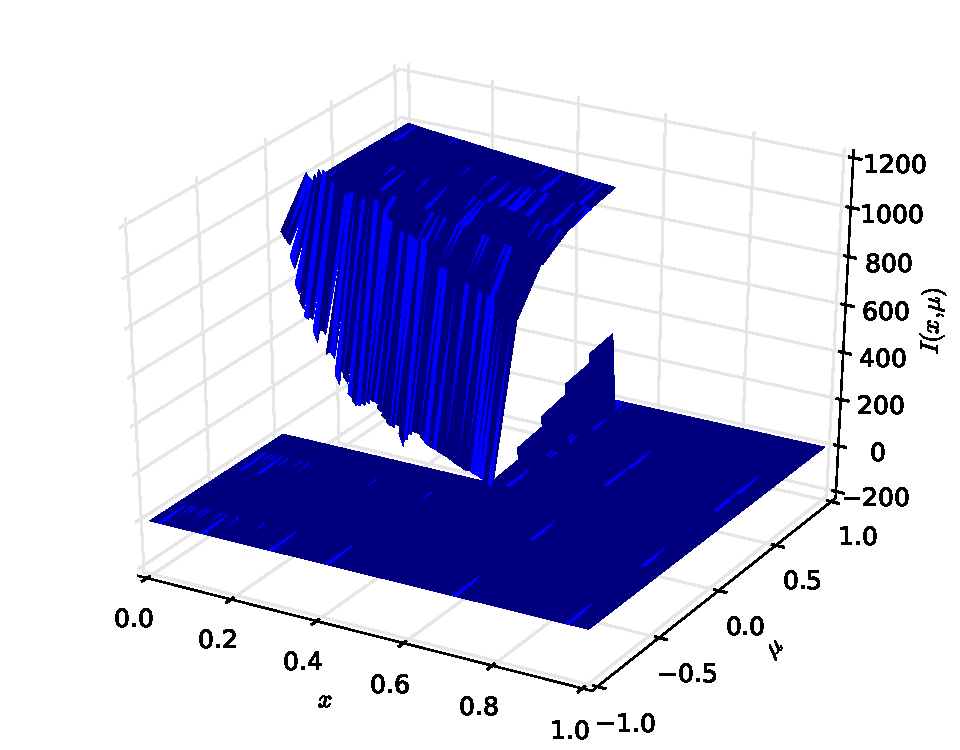
\includegraphics[width=0.99\linewidth]{neut_ang_full.pdf}
    \caption{\label{fig:neut_ang_full} Full plot of $\tilde I(x,\mu)$.}
\end{subfigure}
\begin{subfigure}{0.7\textwidth}
  \centering
  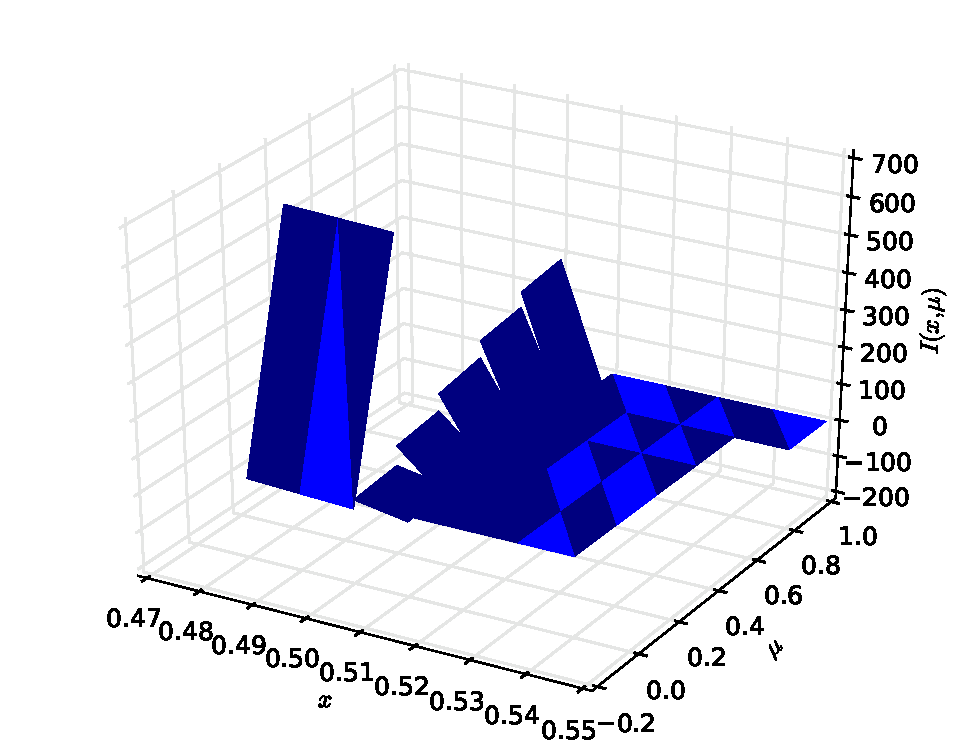
\includegraphics[width=0.99\linewidth]{neut_ang_zoom.pdf}
  \caption{\label{k_200_compare} $\tilde I(x,\mu)$ for cells where $\tilde I(x,\mu)$
  crosses $I_{\min}$.   }
\end{subfigure}
\caption{Plots of $\tilde I(x,\mu)$ for the fixed-source problem.}
\end{figure}

We now test the artificial source fixup and compare to two different cases.  The L$_2$
norm of the error in cell-averaged mean intensities $\|e\|_{a,rel}$ is computed using
Eq.~\eqref{eq:avg_err} from the last time step, averaged over 20
simulations.  Table.~\ref{tab:fixed_source_accuracy} compares 

\begin{table}
    \begin{tabular}{|c|cl|cl|c|} \hline
        Method & \multicolumn{2}{|c|}{$\|e\|_{a,rel}$} & 
        \multicolumn{2}{|c|}{$\|\phi_{HO}-\phi_{LO}\|_{a,rel}$} &\multicolumn{1}{|c|}{FOM}
        \\ \hline 
 Rotate Every Batch &   & ()  &   & () &   \\
 Rotate Last Batch  &   & ()  &   & () &   \\
 Artificial Source  &   & ()  &   & () &   \\ \hline
    \end{tabular}
    \caption{\label{tab:fixed_source_accuracy} Comparison of accuracy in cell-averaged $\phi(x)$ value for
fixed source problem and 100,000 histories per batch.}
\end{table}


